% Michal Kovac's master thesis
%
\documentclass[a4paper,12pt]{book}
\usepackage{pgf}
\usepackage[utf8]{inputenc}
%\usepackage{a4wide}
%% Now, switch on what is appropriate for czech:

% czech quotation marks
% \bq - begin quotation, \eq - end quotation
\def\bq{\mbox{\kern.1ex\protect\raisebox{-1.3ex}[0pt][0pt]{''}\kern-.1ex}}
\def\eq{\mbox{\kern-.1ex``\kern.1ex}}
%\setlanguage{\czech}

{%                                      % Begin a group for which " is active
\catcode`\"=\active                     % Make " an active character
\catcode`\@=11                          % Make @ an active character
%
%  \csdoublequoteson
%
%       This macro makes " an active character, resets the control sequence
%       \dblqu@te to L (left), and defines \dq as a replacement for ".
%
\gdef\csdoublequoteson{%                % \csdoublequoteson enables "
    \gdef"{\czechquotes}%               % Define " as \czechquotes
    \global\catcode`\"=\active%         % Make " an active character
    \global\chardef\dq=`\"%             % Double-quote char. via \dq
    \global\let\dblqu@te=L%             % Always start with a left double-quote
    }                                   % End of macro
%
%  \bq, \eq
%
%      These macros define default characters for czech left and right
%      double quotes. Czech opening quote is created from two commas with
%      kerning depending on fontdimen four parameter of current font.
%      Better solution should be specially designed character with
%      proper kernings; if you have such characters in fonts
%      (e.g. in DC-fonts), use it instead. (e.g. define
%      macros \bq and \eq e.g. \def\bq{\char"130 }
%      in your document/style file-- not in csquote.sty!)
%      Similar solution is used for czech right quote.
%
%      \cs existence test, stolen from TeXbook exercise 7.7
\def\ifundefined#1{\expandafter\ifx\csname#1\endcsname\relax }%
%
%      another macro to be more efficient in time and space
\global\chardef\f@@r=4
%
\ifundefined{bq}%
\gdef\bq{\kern-.25\fontdimen\f@@r\font,\kern-.8\fontdimen\f@@r\font,%
                \kern-.35\fontdimen\f@@r\font}%
\fi
\ifundefined{eq}%
\gdef\eq{\kern-.35\fontdimen\f@@r\font`\kern-.8\fontdimen\f@@r\font`%
                \kern-.25\fontdimen\f@@r\font}
\fi
%
% Macro \uv for other usage of \bq and \eq.
%
\ifundefined{uv}%
        \gdef\uv#1{\bq #1\eq}
\fi
%
% \testquotes macro gives warning if citation span this place
%
\gdef\testquotes{\if R\dblqu@te
        \message{Warning: You forgot right double quote!}%
        \let\dblqu@te=L\fi}
%
%  Define the macro that will be executed whenever " is encountered.
%
\gdef\czechquotes{\protect\czechqu@tes}
\gdef\czechqu@tes{%
        %  If the double-quote is the first character in a new paragraph,
        %  make sure it becomes a left double-quote.  This case can be
        %  detected by checking to see if TeX is currently in vertical mode.
        %  If so, the double-quote is at the beginning of the paragraph
        %  (since " hasn't actually generated any horizontal mode tokens
        %  yet, TeX is still in vertical mode).  If the mode is vertical,
        %  set \dblqu@te equal to L.
        %
        \ifinner\else\ifvmode\testquotes\fi\fi%
        %
        %  Now insert the appropriate left or right double-quote.
        %
        %  If \dblqu@te is L, insert an opening quote and set \dblqu@te to R.
        %
        \if L\dblqu@te\bq\global\let\dblqu@te=R%
        %
        %  Otherwise, save the current \spacefactor, insert '', set \dblqu@te
        %  to L, and reset the original \spacefactor.
        %
        \else%
           \let\xxx=\spacefactor%               % Save the \spacefactor
           \eq%                                 % Insert ending quote
           \global\let\dblqu@te=L%              % and reset \dblqu@te
           \spacefactor\xxx%                    % Reset the \spacefactor
        \fi%                                    % End of \if L\dblqu@te...
        }                                       % End of " macro
}                                               % End of group

\gdef\csdoublequotesoff{%
        \catcode`\"=12%                         % Set " back to other
        }
%
% Czech quotes are default
%
\csdoublequoteson




\newcommand{\uv}[1]{``#1''}

%\pgfdeclareimage[interpolate=true,height=7cm]{faktorial}{faktorial}
%\pgfdeclareimage[interpolate=true,height=7cm]{designimage}{designB}
%\pgfdeclareimage[interpolate=true,height=3cm]{designimageSmall}{designB}
%\pgfdeclareimage[interpolate=true,height=3.5cm]{creatorFactoryimage}{creatorFactory}

\author{Michal Kováč}
\title{User-oriented language for powerful data mining with Ferda}
\date{\today}

\begin{document}
\maketitle

\begin{description}
 \item [Název práce:] Uživatelsky orientovaný jazyk pro řešení úloh DZD
 \item [Autor:] Michal Kováč
 \item [Katedra (ústav):]
 \item [Vedoucí diplomové práce:] Doc. RNDr. Jan Rauch, CSc.
 \item [E-mail vedoucího:] Rauch@vse.cz
 \item [Abstrakt:]
 \item [Klíčová slova:]
\end{description}

\medskip

\begin{description}
 \item [Title:] User-oriented language for solving KDD tasks
 \item [Author:] Michal Kováč
 \item [Department:]
 \item [Supervisor:] Doc. RNDr. Jan Rauch, CSc.
 \item [Supervisor's e-mail address:] Rauch@vse.cz
 \item [Abstract:]
 \item [Keywords:]
\end{description}
\newpage
\tableofcontents
%!--- MARTIN Nikde v obsahu jsem nenasel cast, ktera by srovnavala tvuj postup s jinymi moznymi postupy v DM ci jinde a srovnani v cem je to nase lepsi a horsi. Tohle tam hodne chybi ---
%!--- RE: problem je v tom, ze tu neni zadny alternativni postup, alespon me nic nenapada. Ja proste jen delam programivaci jazyk. Srovnani s jinymi jazyky se deje v ramci psani o tomtom jazyku pri jednotlivych featrach. Druhe misto, kde jsou alternativy jsou ty KDD priklady -- jejich reseni. Zase alternativy se diskutuji v ramci toho konkretniho prikladu. Ale samotne to, ze delam programovaci jazyk, nema alternativu -- co jineho by jsi chtel delat? ---!

\chapter{Introduction}
\section{Zadání}
Východiskem diplomové práce jsou zkušenosti s GUHA procedurami implementovanými v rámci systému LISp-Miner~\cite{GMGC}. Díky jak rozmanitosti vztahů které lze jejich pomocí hledat tak i vzhledem k rozsáhlým možnostem zadávání množiny potenciálně zajímavých vztahů lze pomocí těchto procedur hledat odpovědi na různé analytické otázky formulované způsobem blízkým přirozenému jazyku. Příkladem takové otázky je: \uv{Za jakých okolností a pro které pacienty není pravda, že s rostoucí úrovní cholesterolu roste i úroveň trigliceridů?}. Na tuto otázku lze hledat odpovědi pomocí procedur 4ft-Miner, SD4ft-Miner, KL-Miner i SDKL-Miner. Použitá procedura i způsob nastavení jejích parametrů dává různé možnosti co se týče podrobnosti odpovědi. Zevrubná odpověď na takovouto otázku vyžaduje několik vzájemně provázaných běhů několika procedur. Jednotlivé běhy procedur odpovídají dílčím otázkám indukovaným položenou otázkou.

Lze pokládat řadu podobných otázek které konstituují jistou typovou úlohu. Příkladem podobné otázky k otázce výše uvedené je otázka \uv{Za jakých okolností a pro které pacienty není pravda, že s rostoucí úrovní vzdělání roste i spotřeba vína?}. Pro řešení jedné typové úlohy existuje systém vzájemně provázaných dílčích otázek a ty lze chápat jako příkazy vhodného jazyka, kterým uživatel řídí postup při řešení typové úlohy.

Jedná se o diplomovou práci kategorie \uv{výzkumný problém}. Jejím cílem je stanovit několik typových úloh a pro ně definovat výše naznačený jazyk pro řešení. Jazyk bude založen na použití GUHA procedur implementovaných v rámci systému LISp-Miner, případně na nových vhodných analytických procedurách. Součástí diplomové práce bude i prototypová implementace příkazů tohoto jazyka v rámci systému FERDA~\cite{znalosti2006}.

\section{Reaction to proposal}
!--- MARTIN nove pojmy v teto i v dalsich sekcich by meli byt poprve kurzivou, potom uz normalne, at ctenar vi, ze je to neco noveho v textu a ne nejaky common knowledge ---

The main task of this thesis is to assess a set of several problems in KDD and present a possible solution via a new user-oriented language for the Ferda system. The reach of the present thesis, however, surpasses the assignment in its implications. Instead of a new language specific only for some KDD problems, a new generic language with much wider extensibility and usability has been created as a part of this thesis. The reason for going beyond the task was the author's determination to present a more complex solution to the problem given. 

Instead of presenting first the KDD problems and later describing a new language specific for these problems a new generic language is introduced at the beginning. The generic language resulted indeed from some KDD problems but it is not visible on the result, which is why it is not needed to start with examples in this thesis.

The creation of a new more generic language independent of KDD was established as the first task, followed by demonstration of KDD problems and their solution using the given generic language and special KDD functions in addition. The method used for creation of the new language relied on the principle of other functional languages, while maintaining the basic requirements of recursive countability and the widest possible application on the KDD problems.

!--- MARTIN tomuto odstavci nerozumim ---

There are references from solution of KDD problems to features in the new language which are used for their solution. Therefore it is possible to read problems with their solution first, but it is not recommended for understanding the new language.

%!--- MARTIN vysvetlit asi trosku lip, ctenar nemusi tusit co to je Ferda nebo LISp. Myslim ze Rauch k tomuto odstavci bude mit pripominky :) ---
%!--- RE: cilem tohoto odstavce neni aby ctenar chapal, co je LISp ci Ferda, jen aby pochopil, ze z nejakeho chytreho duvodu "neni splneno" zadani - vlastne je to jen oprava zadani - ve kterem taky neni vysvetleno, co to je LISp ci Ferda ---!

The new implementation of GUHA procedures that has been created as a part of \cite[diploma thesis of Tomáš Kuchař]{thesisKuchar} is used instead of LISp-Miner procedures which have been proposed. The new implementation of GUHA procedures is more generic and better integrated into the Ferda system. Use of the LISp-Miner procedures has been removed from the Ferda system.

\section{Structure}
The thesis is divided into five chapters. The first chapter discuss proposal of the thesis, guides to a solution of the proposal and a structure of the thesis.

The second chapter introduces the Ferda system. First, it discusses the history of Ferda and its implementation. Subsequently, it presents its functional view. The chapter shows that Ferda was from beginning designed for user-oriented functional programming and it describes what was missing in the Ferda system from the point of programming and extensibility before this thesis.

The third chapter goes into more details and describes new features, functions and tools which can help making Ferda better user-oriented programing tool. To start with, it focuses on source files, the basic programming instrument, and how they are organized and how a code can be reused. Then several new basic functions are introduced with description of their pilot implementation. Modern programing methods are discussed in the last part of this chapter. Neither this chapter nor the first chapter are specifically oriented on knowledge discovery or data mining.

The fourth chapter realises the main part of the proposal. It shows examples from KDD and shows how it can be solved in the Ferda system by functionalities introduced in the first two chapters. It also proposes new functionalities specific for KDD.

The last chapter summarizes previous chapters. It lists features which have been implemented as part of this thesis and features which have been proposed only.

\chapter{Basics of Ferda}
This chapter describes the Ferda system. First, it discusses the history of Ferda and its implementation. Subsequently, it presents its functional view. The chapter shows that Ferda was from beginning designed for user-oriented functional programming and it describes what was missing in the Ferda system from the point of programming and extensibility before this thesis.

\section{History}
Michal Kováč, Tomáš Kuchař, Alexander Kuzmin and Martin Ralbovský started to work on Ferda Data Miner in the year 2003. It was been held as a software project for Faculty of Mathematics and Physics of Charles University. The project was lead by doc.~Jan Rauch. The basic aim of this project was creation a of a user-friendly user interface for the LISp-Miner project~\cite{LISp-Miner} in style of visual programming. LISp-Miner is a system which consists of several KDD procedures based on GUHA~\cite{GUHAbook} principle. The Ferda was created with future extensions in mind and the main parts of the application are independent of data mining at all.

The Ferda is a user-oriented application for working with special visual objects called boxes. They are represented by small squares with an image atop. Boxes have sockets and a user can connect other boxes to these sockets. Boxes represent functions, sockets are places for parameters for these functions. Note the used terminology: Ferda Data Miner is the Ferda system with boxes for data mining.

!-- TODO vložit obrázek krabičky --!

In the version 1.x of the Ferda system, the boxes for data mining were written for the LISp-Miner generators. It was hardly extensible, because Ferda is the most strong when a functionalities of modules are distributed under different boxes. In the 1.x version majority of the functionality was in task boxes, other boxes were only really simple, the task boxes read from them settings, created a setting database called ``metabase'' for the LISp-Miner system, executed a procedure of the LISp-Miner system and read hypotheses which were written by the system to the metabase.

Later Tomáš Kuchař as a part of his diploma thesis~\cite{thesisKuchar} wrote his own implementation of additional GUHA procedures for Ferda Data Miner (version 2.x). The new implementation distributed functionalities under different boxes. The new implementation of GUHA procedures is also stronger in the point that it allows disjunctions between atoms in hypotheses~\cite{RalbovskyDisjunction}.

Since the completion of the project, numerous new boxes have been created for special applications like decision trees~\cite{GUHAtrees}, ontology mapping~\cite{thesisZeman} or relational GUHA procedures~\cite{thesisKuzmin}. 

!-- TODO vlozi jeste Martinovu diplomku --!

History of the Ferda system is described in detail in~\cite{RalbovskyHistory}.

\section{Introduction to Ferda}
The Ferda is a client-server application. Client executable is the FerdaFrontEnd.exe and we call this part FrontEnd. There is no single server executable; instead there are more separate modules which all can act as separate applications. FrontEnd communicates with all of them. Some of these modules implement boxes so we call them box modules, other are helper modules like the GUHA mining engine.

The FerdaFrontEnd is a visual application. The main object of Ferda is a project. The project consists of an archive and views. The archive is a place for boxes. Views adds to boxes its placement on a desktop. Desktops are places where boxes are shown with theirs connections, they are shown view. Every box which is in the archive can be either in none or in one or more views.

The FerdaFrontEnd has a menu by which user can for example load or save project, show desktops or open a tutorial. By default, desktops occupy majority of a space on a screen and they are in the center, on the left is archive and list of boxes which can be added to a project, on the right is a property grid, context help and user note.

!-- TODO pridat obrazek Ferdy

Box modules consist of sockets, properties and functions. Sockets are places where you can connect another box module. They represent parameters for functionality of the box module. Properties are also such parameters and can be viewed as a socket, but can be configured both by connecting a box to the socket and by setting the property in the property grid. Every property has in the property grid two lines. One line for setting of the property by the property grid, the second line for setting a boolean value indicating if there should be visible a socket for that property. If it is set to true, the first line is disabled (it means you can not change a value manually) and its value depends on a functions object which is returned from a box which is connected to the socket of that property. Please see figure~\ref{fig:propertyAsASocket}. This has been done in time of the software project Ferda by the author of this diploma thesis, because he had in mind future functional possibilities of Ferda. 

!--- MARTIN toto by chtelo priklad ---

\begin{figure}
	\centering
	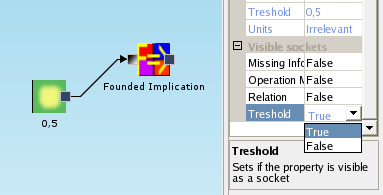
\includegraphics[width=7cm]{property_as_socket}
	\caption{A property as a socket}
	\label{fig:propertyAsASocket}
\end{figure}

A box module has a method which returns a object called functions. This object represents the functionality of the box module. A box module has also an identifier, an icon, a SVG design, names of categories, box modules asking for creation, actions, a name of property driving label and a dynamic help.

\section{Ferda as a programming language}
\newtheorem{mydef}{Definition}

This section describes boxes as a function, formalizes boxes and introduces a new method of writing a connections of boxes.

The main concept of Ferda is to be user-oriented functional language. The basic abstraction is that a box is a function and sockets are properties of that function. There is no need to talk about properties, because properties are also accessible by sockets. It is typed language. The box returns an object called ``functions''. A socket specifies which types of functions can be connected to the socket. A box also specifies which types of functions it returns. Types of functions are called ``Ice identifiers''. One object can have more these types.

Ferda is environment for the language. We will call the language of Ferda the Ferda language. The language has its syntax and semantics. Syntax is in the Ferda science about boxes and connections regardless their meanings. The syntax specifies is specification how can a connection look like. The semantics of the Ferda is specification how to count a result of connection of boxes. Source codes of the Ferda language are connections of boxes. Source files of the language are project files of Ferda.

\subsection{Formalization of boxes}
Let us create a formalization of basic objects of the Ferda user-oriented language. It will not be used later in the text, but it will show more precise declaration of the language.

%To be more precise, box can be not only viewed as one function, but as set of functions. As written above, box returns object functions. Therefore every method of such object can be viewed as a separate function. Box can also return different functions object depending on its parameters. We can define basic objects of the Ferda user-oriented language.

\begin{mydef}
Box is $\left<S,F\right>$ where
\begin{itemize}
	\item $S$ is a set of sockets
	\item $F$ is a set of functions which use sockets from $S$
\end{itemize}
\end{mydef}

\begin{mydef}
Socket is $\left<n,T\right>$ where
\begin{itemize}
	\item $n$ is socket name
	\item $T$ is a set of box types
\end{itemize}
\end{mydef}

\begin{mydef}
Let us have a predicate $hasIdentifier(f,i)$ where $f$ is function and $i$ is an ``Ice identifier''
\end{mydef}

\begin{mydef}
Box type is $\left<i,S\right>$ where
\begin{itemize}
	\item $i$ is an ``Ice identifier''
	\item $S$ is a set of $\left<n,i\right>$
	\begin{itemize}
		\item $n$ is socket name
		\item $i$ is an ``Ice identifier''
	\end{itemize}
\end{itemize}
\end{mydef}

\begin{mydef}
Box $B=\left<S,F\right>$ is of type $A=\left<i,Z\right>$ (we will call it predicate $isOfType(B,A)$) iff 
\begin{enumerate}
	\item $(\forall \left<n,j\right>\in Z)(\exists \left<m,T\right>\in S)(\exists \left<y,W\right>\in T)(m=n \wedge j=y)$
	\item $(\exists f\in F)(hasIdentifier(f,i))$
\end{enumerate}
\end{mydef}

\begin{mydef}
A box $B=\left<S,F\right>$ can be connected to a socket $s=\left<n,T\right>$ iff $(\exists t\in T)(isOfType(B,t))$
\end{mydef}

\subsection{Description of method of writing}
\label{sec:formalisation}
A new type of writing functions in a text is described in this section. That type of writing is used in the next chapters. On many places a screenshots of Ferda can be used as a presentation of functions, but on them you do not see every settings of the connections. For example you can not see properties of all boxes. The written connections will be also shortened.

Because the Ferda language is a functional language the standard prefix notation suggests itself. The problem is that parameters are in the standard notation in brackets divided only with comas. Order of parameters describes which parameters which are. But parameters of sockets does not have any order. The only identification of them are their names. So we will prefix parameters with their names and the symbol of equality. Let us describe the notation.

If a box $B$ has all it's sockets unset (all properties has its default value) we will write such connection
\begin{equation}
B()
\end{equation}

If a box $B$ has some of its sockets set, but it is not important for the text we will write such connection
\begin{equation}
B(\dots)
\end{equation}

If a box $B$ is connected to a socket with name ``socketName'' of box $C$ we will write such connection
\begin{equation}
C(socketName=B())
\end{equation}

If a box $B$ is connected to sockets with names ``socketName1'' and ``socketName1'' of box $C$ we will write such connection
\begin{equation}
C(socketName=B(), socketName2=B())
\end{equation}
or we can name a part of connection and reuse it in next connections
\begin{equation}
B=B(); C(socketName=B, socketName2=B)
\end{equation}
We will call in this text instances of boxes by a name of their type, for example ``$Table()$''. If in the connection are more boxes of the same type we will distinguish them by their indexes, for example ``$Table_1()$''.

\section{Programmers view of the Ferda system}
Programmers of the Ferda system need to have deeper knowledge than the users. This thesis changes how Ferda works inside, so we are going to describe the design of Ferda from the programmers view.

Base parts of Ferda have been written in C\# 2.0. The Ferda runs on both .NET Framework and Mono. Some modules use also the Java platform. The Ferda uses middleware Internet Communications Engine for a communication between its modules. Every module can be written in different language and run on different computer. For easier development, many third party libraries and applications are used -- mainly NAnt, NUnit, NDoc, Netron Graphic Library and DockDotNet library.

!--- MARTIN Zde vsude je treba dodelat odkazy na weby --- 

The Ferda is under second version of General Public License. It allows everybody to use it for free, redistribute it, change the code (providing the results are still under the General Public License).

!--- MARTIN Zde vsude je treba dodelat odkazy na weby ---

The aim of the Ferda project was to create application which is internationalized, well documented, modular, user-friendly and conforms Microsoft standards in user experience.

\subsection{Architecture of the Ferda system}
\begin{figure}
	\noindent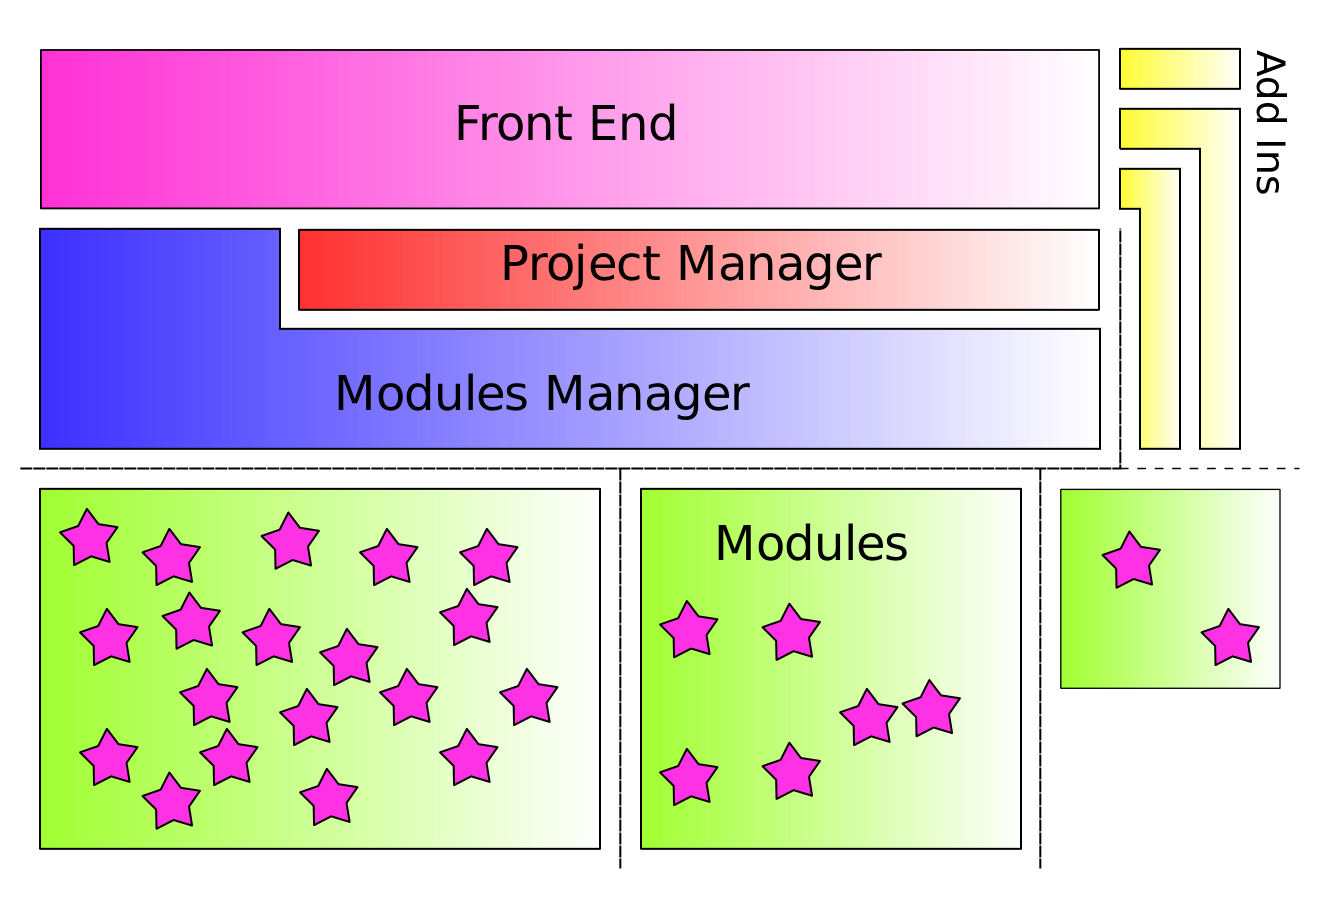
\includegraphics[width=1\textwidth]{designB}
	\caption{Architecture of the Ferda system}
	\label{fig:architectureFerda}
\end{figure}

Let us describe architecture of the Ferda system. Please see figure~\ref{fig:architectureFerda}. The main application is the FerdaFrontEnd.exe. It contains main visual parts of the Ferda system.

FrontEnd uses the assembly FerdaModulesManager.dll for communication with modules. This assembly is abstraction layer so that FrontEnd does not know that modules are not implemented locally (it hides Internet Communications Engine).

Another assembly that is used by FrontEnd is the FerdaProjectManager.dll, which controls projects.  This manager is able to load a project from XML file and save it to XML file.

FrontEnd also loads add-ins. Add-ins can extend functionality of FrontEnd in many ways. It is mainly used for modules for interaction and setting modules. Modules for interaction work on top of some box module. It for example shows results of functions returned by the box module in user comprehensible way. Setting modules are used for helping with setting nonstandard properties of boxes.

The communication between FrontEnd and modules and between modules itself is feasible via the \emph{Internet Communication Engine} (Ice). Ice is a strong modern middleware. Thanks to the usage of Ice, Ferda is independent of both language and framework and it allows us to run different modules on different computers, without having big computational overhead. It can be also used for distributed computing. Every Ice interface is defined in a special language \emph{slice}. On the figure~\ref{fig:architectureFerda} the Ice is represented by the lines.

IceGrid application, which manages available modules and loads them on demand, runs on a network. Modules manager uses these applications for getting modules. This application is part of Ice, so on the figure it is also represented by the lines.

\subsection{Creation of new boxes}
This section of the thesis is not crucial for understanding of a text later. It describes how modules create internally new instances of boxes. This part can be useful for a new programmer of boxes.  

Because use of the Ice a creation of new boxes is more complicated. There is a need of distributed garbage collection. Please see figure~\ref{fig:creatorFactory}. Every box module implementation has its factory class. This factory class creates box module instances. There is one more layer -- every box module factory has its factory class, we call it box module factory creator, which is a singleton.

\begin{figure}
	\noindent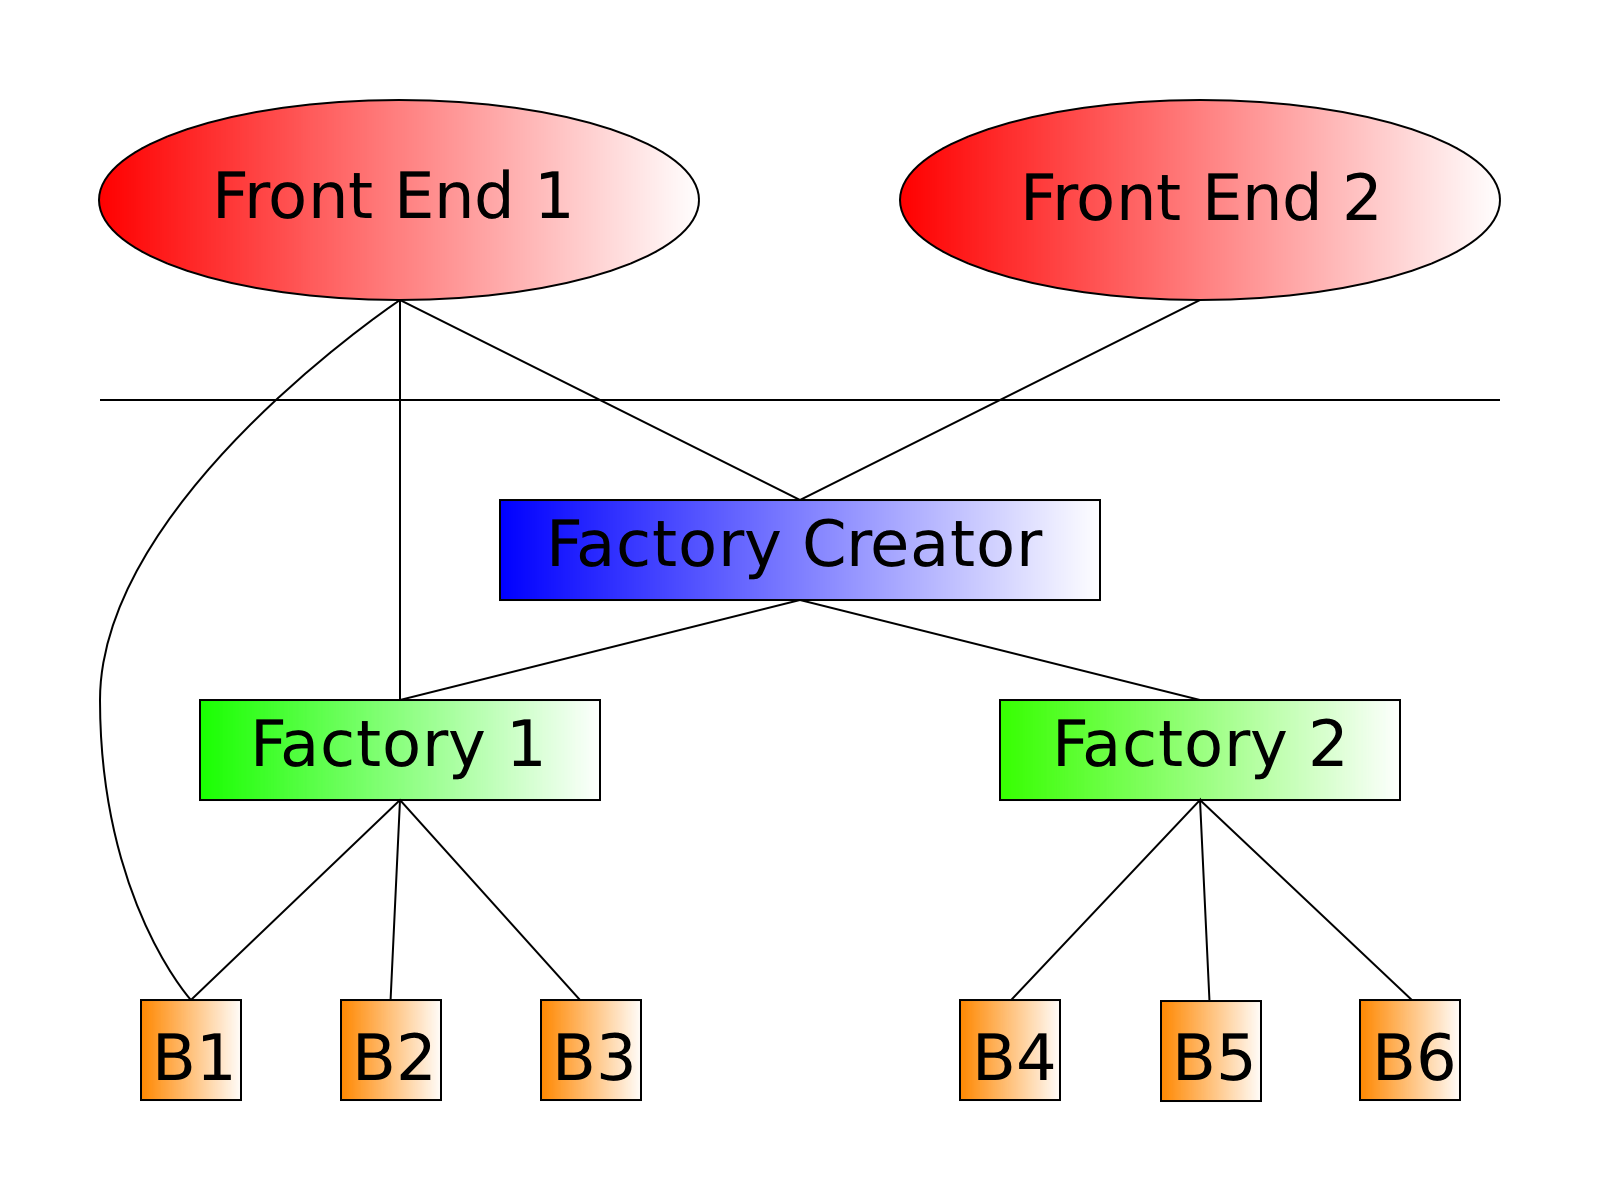
\includegraphics[width=1\textwidth]{creatorFactory}
	\caption{Creation of new boxes}
	\label{fig:creatorFactory}
\end{figure}

FrontEnd asks a box module factory creator for creation of only one box module factory for one box class. The creator has methods independent of both instance of the box module and FrontEnd connected. A factory has methods independent of box modules, but dependent on FrontEnd (for example localized names of properties). If FrontEnd is not connected for longer time, all factory instances and box module instances are destroyed.

Word ``box'' in this thesis may mean two different things according to placement -- a box module or a box instance. A box module represents implementation. It has one instance of Ice box module factory creator interface which is registered in a IceGrid. A box instance is instance of Ice box module interface. One box module can have more box instances.

\chapter{New features for visual programming}
This chapter describes the Ferda system as a visual programming language. It presents possible objects of the language and tools and utilities for the programming.

\section{Source codes and reusability}
\label{sec:reusability}
Every programming languages have ways how to reuse a code. This part of thesis is about ways how to make a programming in Ferda efficient. Need of rewriting a code and missing user specified structure in boxes could release in a usability problem of any language in Ferda. Several ways how to solve these problems will be described with one implementation of such solution.

\subsection{Project import}
The simplest way is to copy the source code to different place and use it for different project. The same is possible in Ferda, you can copy a project file and reuse it.

With standard textual source code it is easy to merge the code from more sources. You can do it with the Ferda project, but you must merge a code in a project files manually in a text editor. The merging is not an easy process so it is not so much user-friendly way.

It would be convenient have a functionality in Ferda that would allow us to import some or all boxes from one project into another one. One way to achieve that would be adding a new item "import project\dots" to the Ferda menu. Therefore, if a user selected this item, a dialog for selecting a project file would open. Having selected a project, the dialog with boxes in selected project should be shown. The user could select boxes which he would want to import. The last step would be the actual import of selected boxes.

Let us discuss the dialog box where a user could select boxes. To chose whole functions, seeing the dependency among boxes would be crucial. However, should the user selects to import a box without a box connected to this box, the box would be imported, but the result of such box could differ significantly from the situation before. On the other hand, such choice could be purposeful should the user want to connect to that box some box from original project.
% - zlepsit citelnost

% (or box connected to box connected to\dots connected to this box -- I will call this indirect connection) 

\subsection{Project using}
The source code of one application is usually not written only in one source file, but in various. There are more ways in programming languages how to achieve this. One way typical for compiled languages is compilation of application from more source files from the beginning. A compiler has a set of files as an argument. The other way, specific for interpreted languages, is an import of another file into the source file. An advantage of this approach is that the imported file is loaded when it is used - so the file can be created a short time before usage. It allows us to write code which loads every file in some directory so that it can be used for plug-ins. Even compiled applications have a way how to achieve this functionality. Compiled applications can use libraries (or assemblies or modules) which can be loaded dynamically on demand. It can be also used for loading a source file on demand if a compiler for that language is available in machine where the application is being executed.

If we wanted to add this to Ferda, project would have to have a new attribute defining the using of other projects. Boxes from these project should be read only - no change of properties and boxes connected to their sockets would be available. Also, the origin of each box should be clearly traceable.

Nevertheless, the import itself of projects into other projects presents a demanding situation. Let us illustrate this on the following example: let us have two imaginary projects, $A$ and $B$, with corresponding boxes, $A$ and $B$. The project $B$ is imported by the project $A$, and the box $B$ is connected to the box $A$ in the project $A$. Even if we remove the box $B$ in the project $B$, maintaining the information about the former connection to already non-existent box $B$ in the project $A$ would facilitate the reversible operation in case we needed to add the box $B$ back into the project $B$. This would allow us to change boxes and therefore functionalities.

Let us discuss possible implementation of such imports. Information about imported projects should be serialized to a project files. In the project file should be a section with paths of imported project files. Boxes which are used from other projects should not be serialized, but connections of these boxes in the project and theirs positions on desktops should. It raises a question how to identify these boxes. The first solution which comes into consideration is to use as identification a pair project identifier of a box and an identifier of an imported project. Such solution would have problems which should be resolved.

At this time boxes are identified in one project by project identifier. The project identifier is an integer which grows from one up without the awareness of the user. If the user removed a box with last project identifier, exited Ferda, started Ferda, reopened the project and added a new box, the new box would have the same project identifier as the removed box had. If we liked still to use project identifier as identification of boxes we should avoid this by serializing the last used project identifier in the project. To be able to replace a box, it is vital the user be able to chose the project identifier.

%tady by mohlo byt jak by melo vypadat menu a ze maji byt videt importovane veci v archivu
\subsection{Defining function}
versus lambda expression - the same
\subsection{Name spaces}
\subsection{Network archive}
Another way how to reuse a box can be to copy it from another project. Let us have a new place where you can place boxes which you want to reuse. Such place can be on network and more users can place their boxes there and reuse them in other projects. They can use such place to move their work to others. Let us call this place a network archive.

\subsubsection{Implementation}
As part of this thesis, the present author has created a simple implementation of such network archive. The main part is a Ice service which is running somewhere on network. It has simple definition in slice:
\begin{verbatim}
interface Archive {
	/**
	 *
	 * Adds a box with connected subboxes to the archive
	 *
	 **/
	void addBox(Box boxValue, string label)
		throws NullParamError, NameExistsError;

	/**
	 *
	 * Removes the box from archive
	 *
	 **/
	void removeBox(string label)
		throws NameNotExistsError;

	/**
	 *
	 * Gets box which is in the archive
	 *
	 **/
	Box getBox(string label)
		throws NameNotExistsError;

	/**
	 *
	 * Gets labels of boxes in the archive
	 *
	 **/
	idempotent Ferda::Modules::StringSeq listLabels();
};
\end{verbatim}

The Network archive is a collection of boxes (with all theirs sub-boxes -- boxes connected both directly and indirectly to that box). Each box is identified with some label. You can add a box and remove a box, get information about a box and list all labels in the collection. The collection is serialized on a disk every time it changes. After startup of the service, it loads the last serialized version.

From the user perspective the network archive is a new panel with list where you can copy a box to. Please see figure~\ref{fig:addToNA}. 
\begin{figure}
	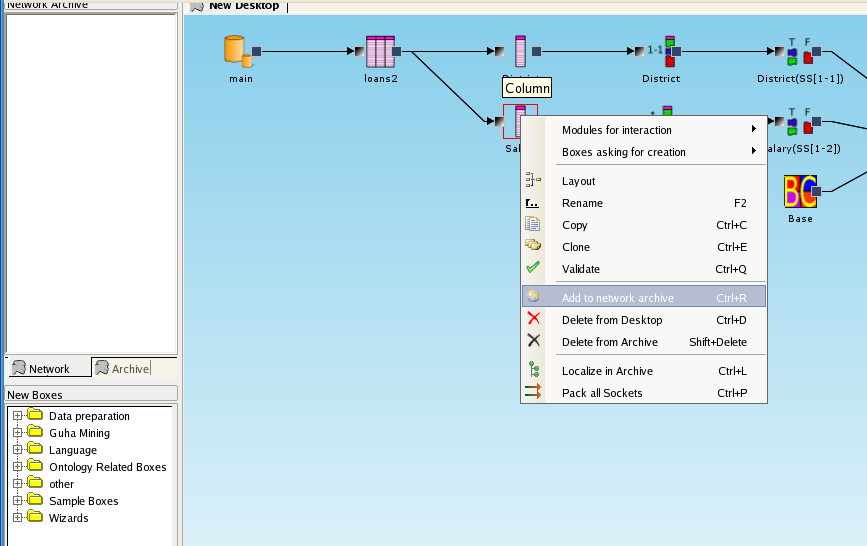
\includegraphics[width=1\textwidth]{add_to_network_archive}
	\caption{Add a connection to the network archive}
	\label{fig:addToNA}
\end{figure}

It will ask the user to enter a label after dragging a box from desktop to the network archive. Please see figure~\ref{fig:setNameInNA}.
\begin{figure}
	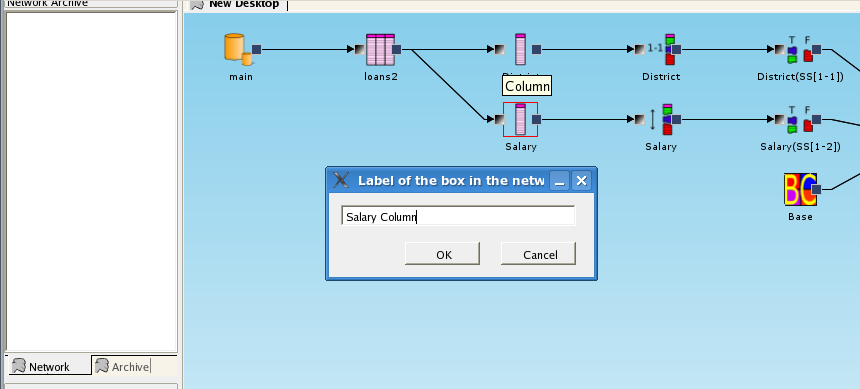
\includegraphics[width=1\textwidth]{set_name_of_box_in_network_archive}
	\caption{Set a name of box in the network archive}
	\label{fig:setNameInNA}
\end{figure}

After that a new item with selected label should be visible in the list. Please see figure~\ref{fig:addedToNA}.
\begin{figure}
	\centering
	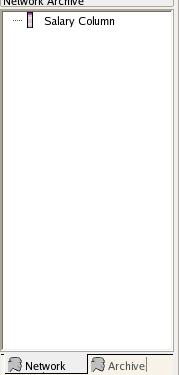
\includegraphics[height=7cm]{network_archive_box_added}
	\caption{New box added to the network archive}
	\label{fig:addedToNA}
\end{figure}

The user can then go to another computer which uses the same network archive and drag the box from network archive to another project. It should create a new copy of the box with all its sub-boxes on the desktop. Please see figure~\ref{fig:dragFromNAToDesktop}.
\begin{figure}
	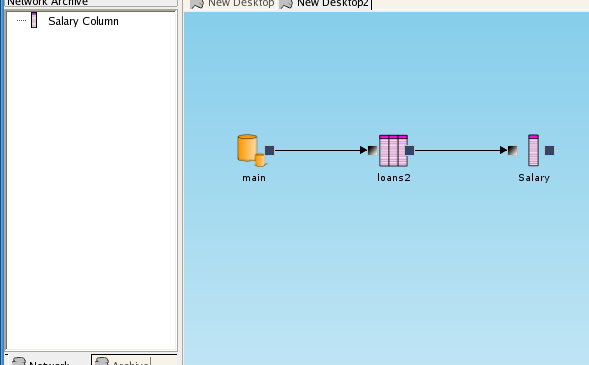
\includegraphics[width=1\textwidth]{network_archive_drop_to_desktop}
	\caption{Drop box to a desktop from the network archive}
	\label{fig:dragFromNAToDesktop}
\end{figure}

He can also remove the box from the network archive. Please see figure~\ref{fig:removeFromNA}.
\begin{figure}
	\centering
	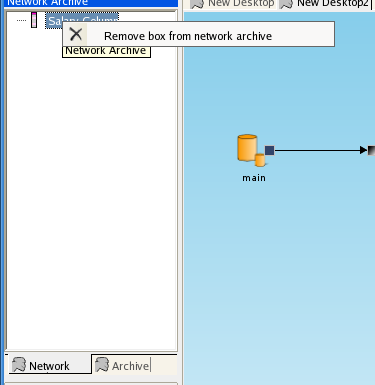
\includegraphics[height=7cm]{network_archive_remove_box}
	\caption{Remove box from the network archive}
	\label{fig:removeFromNA}
\end{figure}

\subsubsection{Future enhancements}
Organizing boxes in network archives into some structure would facilitate the work. It could be one-level structure (labels) or tree-structure like in directories. Another enhancement would be to add user rights to these labels.

Easy thing to do is to allow the Ferda FrontEnd to work with more network archives.

\subsubsection{Summary}
The network archive is a new place where the user can store connections. It is independent of projects. One network archive can be accessed from more computers. It is a way how to move connections from one project to another.

\subsection{Summary}


\section{Functional languages}
We have choose in Ferda that boxes represents functions and the language of Ferda system is functional. Many visual programming languages exist~\cite{WikiVisualProgrammingLaguage}, but we don not know about any which is functional. Most of these languages are dataflow, workflow or object-oriented languages. The biggest difference between these languages and a functional language is that in a functional language a result of program is a return value of some function. In a visual programming language it means that a execution of a program is a tree of boxes where root of the tree is an endpoint of the execution. The tree is similar to the connection of the boxes on a desktop, only cycles are expanded and two uses of the same box are in the execution two boxes. In workflow and dataflow languages there can be more endpoints. In the object-oriented languages there is one main object which is responsible for a execution, but from the connection of boxes it is not possible to know an execution plan.

When Ferda has been designed we have taken a look on other two data-mining tools -- Weka and Clementine. The first is free the second is commercial. Both Weka and Clementine have something like workflow visual programming language.

We are able to naturally represent objects of interest with a functional language. Ferda has typically more boxes for the same task than some workflow oriented visual programming language. Workflow and dataflow oriented languages have more settings in a property grid and dialog boxes. So we can say that the language of Ferda is more low level.

Several reasons guided authors of Ferda to make the language in Ferda functional. GUHA~\cite{GUHAbook} is a theory which has its own logical calculus. Formulas of any calculus are mostly written like functions. Semantic of formulas can be seen as a value of the functions. It means that a calculus can be seen as a functional language. Big similarity between functions and formulas can be also found in constructions of transparent intensional logic~\cite{webTIL}. Both have as a base typed lambda calculus~\cite{WikiLambdaCalculus}. Functional language is in many ways close to the natural language.

LISp-Miner~\cite{LISp-Miner} has mostly for each type of GUHA method three programs -- the first for setting of the task, the second for generating of results and the third for browsing the results. The partioning has been affected by work flow of data mining. If we had done Ferda workflow oriented, it would have three boxes for one task which would correspond to the three programs of LISp-Miner. Ferda has advantage of reusability compared to LISp-Miner, because setting of a task is done by many boxes. It would not have if we had done Ferda workflow oriented. 

Functional languages are typically full featured scripting languages. They are part of many scientific applications, because writing to such languages is similar to functions written to scientific books. So scientists used to use such languages. Workflow and dataflow languages are typical for concrete problems. The set of rich boxes for the concrete problems are prepared in such languages. Typically they are strong for the things they were designed to do, but it is hard to use them by a user for something else.

This thesis brings some new boxes, which are described in the section~\ref{sectionNewBoxes}. Ferda is full featured language thanks to these boxes. It means that it can be used for most of tasks on a computer. The language is recursively enumerable.

\section{Language boxes and expressions}
\label{sectionNewBoxes}
Every programming language has from beginning at least small set of functions. Also it has some way how to use these functions to create more complex ones. Such an instrument has been created for Ferda as crucial part of this diploma thesis. New language boxes are presented at this part of thesis. Data-mining examples which use these boxes are shown in the chapter~\ref{chap:KDDExamples}.

\subsection{Constants}
The Ferda language is a typed language. It means that functions in Ferda return values of some type. Easiest functions are constant functions which return specified value. There are at least two ways how to achieve this by box semantic. One way is to create a specific box type for each type of constants which returns that specific type. This type has been created in Ferda as a part of this thesis.

!-- TODO přidat obrázek --!

The other type is to create one box type which has one property for specifying a type and dependent on it it would have a second property with a value of a specified type. It would return that value.

\subsection{Boxes for math}
Mathematical expressions are really necessary for programmers, statistics and analytics. Support for them is important. New boxes for basic mathematic functions have been added.

\subsubsection{Binary operation}
New boxes for basic binary operation have been added. It has three properties. First two, called ``value1'' and ``value2'', are arguments of an operation. Theirs type is double. The last property is type of operation ($+$, $-$, $*$, $/$), it is called simply ``type''. Result of such operation is always double. Please see figure~\ref{fig:boxBinaryOperation}. In the figure you can see that ``value1'' and ``value2'' properties are set by sockets.
\begin{figure}
	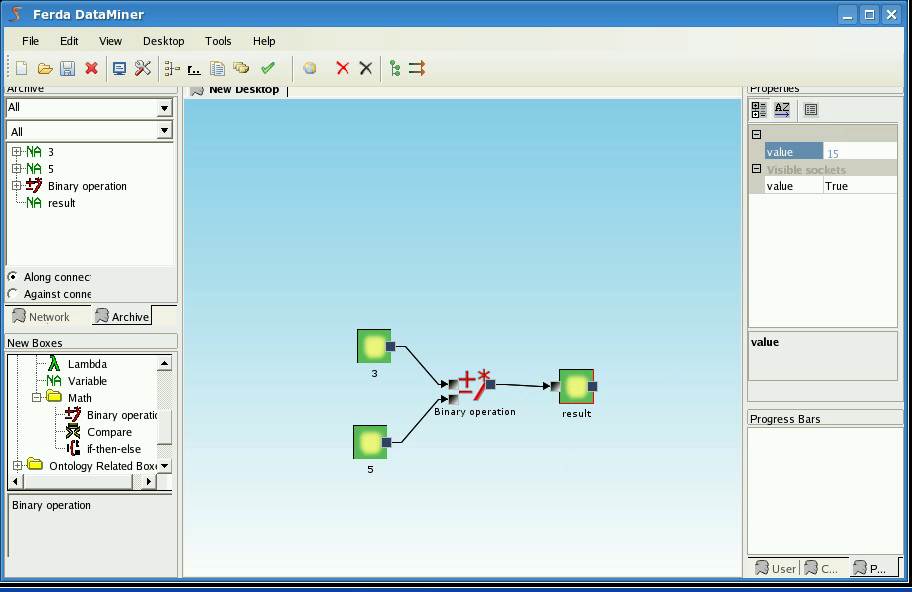
\includegraphics[width=1\textwidth]{binaryOperation2.png}
	\caption{Binary operation}
	\label{fig:boxBinaryOperation}
\end{figure}

Such box can not be used for setting up a integer properties, even if it sums only integers, because it always returns double. One way how to overcome such problem is to introduce a new convert box. The second way is to change the behavior of the binary operation box. It would return an integer if it summed two integers. Similarly it would return a float if it summed an integer with a float. Different operation types would behave different as is it standard in other languages. Such function would be less efficient, but more useful.  

There is no need to have one box for all operations. There can be also as many boxes as many operations are. Let us describe how to create for example a plus box. There are more possibilities how to do it. It has been already described in~\cite{znalosti2006} on a plus box. There could be plus box which has two properties ``value1'' and ``value2'' like the binary operation box. But there could be also a plus box which has only one socket ``arguments'' -- the box would sum all boxes connected to this socket. It means less boxes on a desktop when summing more numbers. Also it adds an easy way how to sum sequences of numbers which are described in the section~\ref{sec:sequences}. But even without such box we are able to do it (for example thanks to head/tail box which is described in the same section), only it is complicated.    

\subsubsection{Comparison}
Comparison functions are functions of two arguments which return a boolean value. As part of this thesis a compare box has been created which has three arguments. First argument is type of comparison function, next two arguments are doubles. This box has implemented basic mathematic comparisons ($<$, $>$, $<=$, $>=$, $=$, $!=$). Please see figure~\ref{fig:boxCompare}.
\begin{figure}
	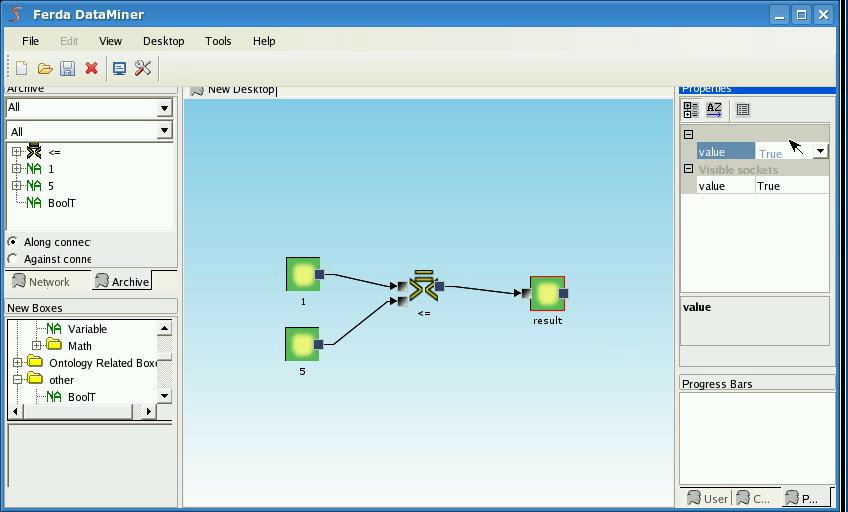
\includegraphics[width=1\textwidth]{compare2.png}
	\caption{Compare}
	\label{fig:boxCompare}
\end{figure}

It is possible to create also boxes specific for every comparison function like has been described for the binary operation box.

\subsubsection{If expressions}
If expression is a function which has three arguments. The first argument, called ``if'', is of boolean type. It returns value of the second argument, called ``then'', if the first is true, otherwise it returns the value of the third argument, called ``else''. Such new box, called ``IfThenElse'' has been created. Please see figure~\ref{fig:boxIfThenElse}.
\begin{figure}
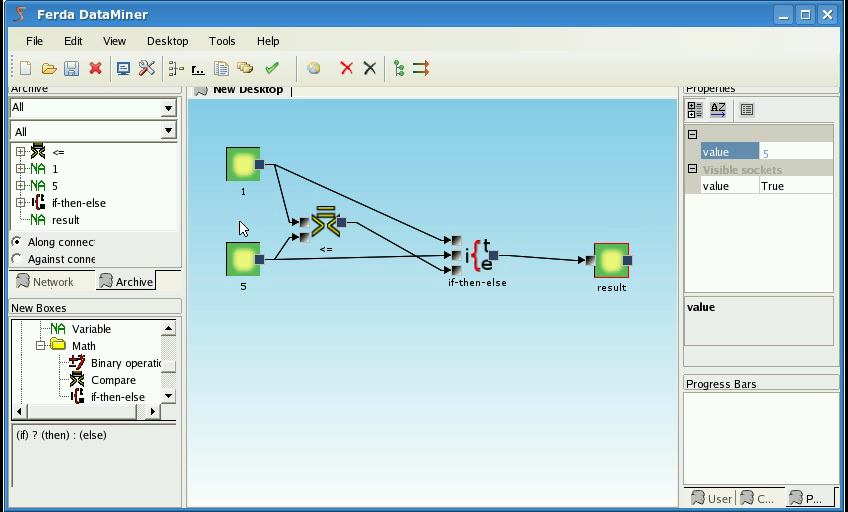
\includegraphics[width=1\textwidth]{ifthenelse2.png}
	\caption{If expression}
	\label{fig:boxIfThenElse}
\end{figure}

Important fact is that if the ``if'' argument was true, the function in the ``else'' socket would not be counted. Similarly if the ``if'' argument was false, the function in the ``then'' socked will not be count. It means that the not counted function can count indefinitely, but the IfThenElse box can return a value.

\subsection{Lambda expression}
Lambda is one of the most important expression for functional languages. Its base is in the lambda calculus. Mathematics many times define a function which they later use. For example see definition of this plus one function
\begin{eqnarray*}
f(x)&=&1 + x\\
y&=&f(9)
\end{eqnarray*}
This equations gives to the $y$ value $10$. In the lambda calculus it equals to this expression
\begin{eqnarray*}
f&=&\lambda x.(1+x)\\
y&=&f(9)
\end{eqnarray*}
The naming of functions is not necessary, it can be also written as $(\lambda x.(1+x))(9)$. Lambda can be seen as a function which has two arguments -- the first argument is set of variables and the second argument is a expression which uses these variables. It returns a function from the variables to the value of the expression after setting up the variables.

Mathematics can also define recursive functions like factorial
\begin{eqnarray*}
f(0)&=&1\\
f(x)&=&x * f(x - 1)
\end{eqnarray*}

The same thing can be done in functional languages with lambda expression. Plus one function will be presented there in more languages with use of lambda expression. Let us show the first example not on a functional language but on a structural one with functional aspects. Such language is the C\# 3. Lambda expression is in the C\# 3 done by operator $=>$:

\begin{verbatim}
public delegate int function(int x);

public static void Main(string[] args)
{
  function plusOne = x => 1 + x;
  var a = plusOne(9);
  System.Console.WriteLine(a);
}
\end{verbatim}

F\# is another language which is translated to IL of .NET framework, but it is a functional language. The lambda expression is done by the let operator there:
\begin{verbatim}
let onePlus x = 1 + x
do printf "%s" (onePlus(9)) 
\end{verbatim}

The last example is written in more commonly used functional language today, in the Python. There is used the ``lambda'' keyword:
\begin{verbatim}
plusOne = lambda x: 1 + x
print plusOne(9)
\end{verbatim}

A new lambda box has been created as part of this thesis. It has socket ``Function'' and a property ``VariablesCount''. Type of this property is integer. There are as many socket pairs variable, value as big the value of this property is. It is first box in Ferda which has dynamic sockets. Such think has been designed in the beginning of Ferda, but because it have not been used, some changes were needed to the core of Ferda to make it running.

Please see figure~\ref{fig:boxLambdaBasic}. The ``Function'' socket represent the expression from the lambda. The ``VariablesCount'' is set to zero in this connection. It means that the lambda returns the same thing which is connected to the ``Function'' socket. In this example the result is six represented as double. 
\begin{figure}
	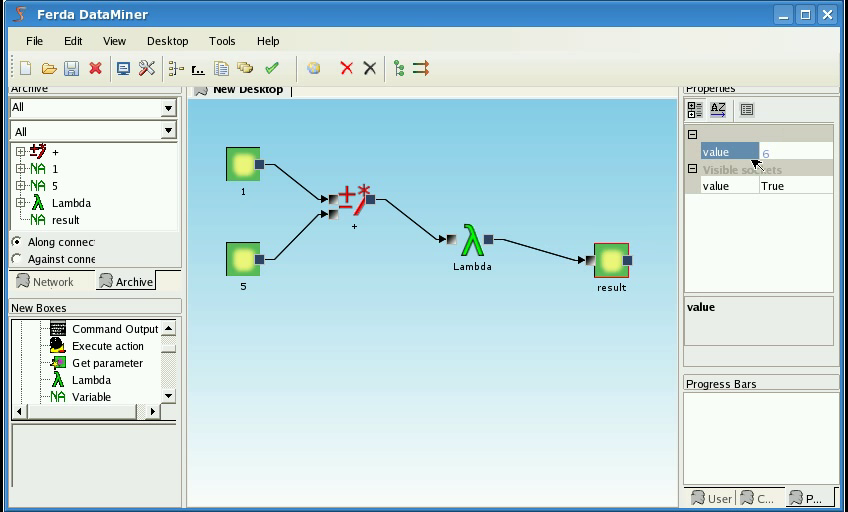
\includegraphics[width=1\textwidth]{lambdaBasic2.png}
	\caption{Lambda without arguments}
	\label{fig:boxLambdaBasic}
\end{figure}

Please see figure~\ref{fig:boxLambdaOnePlus}. It shows the same example in Ferda as we have seen in the previous examples in other languages -- the one plus function. The ``VariablesCount'' is set to one in this connection. It means there are sockets ``Variable0'' and ``Value0''. The box with value five is used there as a variable. The box with value nine is the value of variable. So the result of such connection should be ten.
\begin{figure}
	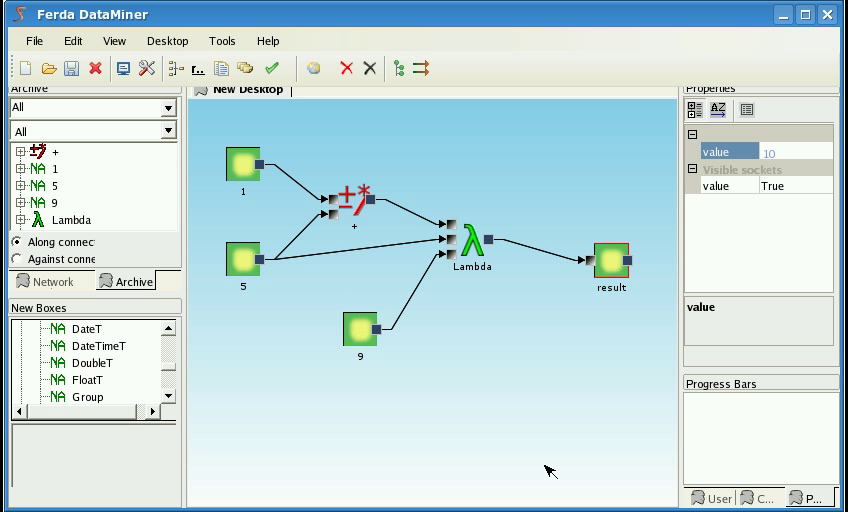
\includegraphics[width=1\textwidth]{lambdaBasic3.png}
	\caption{Lambda with one constant parameter specified}
	\label{fig:boxLambdaOnePlus}
\end{figure}

The type of boxes which can be connected to the ``Value0'' socket are determined by the types of box which is connected to the ``Variable0'' socket. There can be connected more boxes to the ``Variable0'' socket. Then the determined type is intersection of types of that boxes.

It is possible to use as a variable not only a variable box, but any box. To that box can be something connected. It adds possibility of easy writing a recursive function. It will be describe later.   

\subsubsection{Implementation of the lambda box}
If the lambda box is asked for its functions interface it will clone the connection which is in the ``Function'' socked, only instead of boxes which are connected to some variable socket it places there cloned connection to value socket of that variable. After that it returns functions of the main box from the connection.

The cloning is not done in the lambda box, but the project manager is used. Its interface has been extended for cloning functionality as part of this thesis.

In the lambda calculus it is possible that the variable is also non-constant function. For example:
\begin{equation}
\lambda x.(1+x(5)))(\lambda y.(1+y))
\end{equation}

It is not possible with the implementation which is done in Ferda, because the implementation replaces variables with cloned values without reconnecting to the cloned value connections which have the variable. Such thing can be implemented, but there are several complication which must be overcame. One of these is that the lambda box should be able to name its value sockets -- so that it is possible to create a lambda box with the same box type as has any other box.

The implementation has one problem, which is not easy to fix. The cloned boxes are not released until the end of FrontEnd application even if they will not be used and every time any box ask for functions interface of the lambda, new cloned boxes are created. It means amount of used memory raises when the lambda box is used. It is not easy to fix, because today there is no information when a box will not use a functions interface any more. Adding such information to Ferda means changes to almost all boxes.

There is also one performance problem. Let us have function $\lambda x.(x*x)$. If you called in most of functional languages such function with parameter $1+1$, it would firstly count $1+1$ -- two, and later it passes two as the $x$ -- so it counts than $2+2$. In Ferda such function created by a lambda box counts $(1+1)*(1+1)$. It means the plus operation is counted twice. This problem grows when the lambda is used for a recursion. A generic fix is problematic, because in Ferda are functions which can not be stored in a simple class and the connection to other boxes is necessary. For simple types there can be created some cashing mechanism.

\subsubsection{Example usage of lambda -- factorial}
Let us show you how the lambda can be used for a recursive function. On of simplest recursive function is a factorial. Simple structural version of that function in the C\# language is: 
\begin{verbatim}
public static int Factorial(int x)
{
  if (x == 0)
  {
    return 1;
  }
  else
  {
    return x * Factorial(x - 1);
  }
}
\end{verbatim}
	
The better implementation of factorial in C\# is using if expression:
\begin{verbatim}
public static int Factorial2(int x)
{
  return (x == 0) ? 1 : x * Factorial2(x - 1);
}
\end{verbatim}

The factorial in the Python language can be implemented this way:
\begin{verbatim}
fac = lambda x: x == 0 and 1 or x * fac(x - 1)
\end{verbatim}

And the last implementation in the F\# language:
\begin{verbatim}
let rec factorial n =
    if n=0 then 1 else n * factorial(n - 1)
\end{verbatim}

Please see figure~\ref{fig:factorial}. That figure shows an implementation of factorial in Ferda.
\begin{figure}
	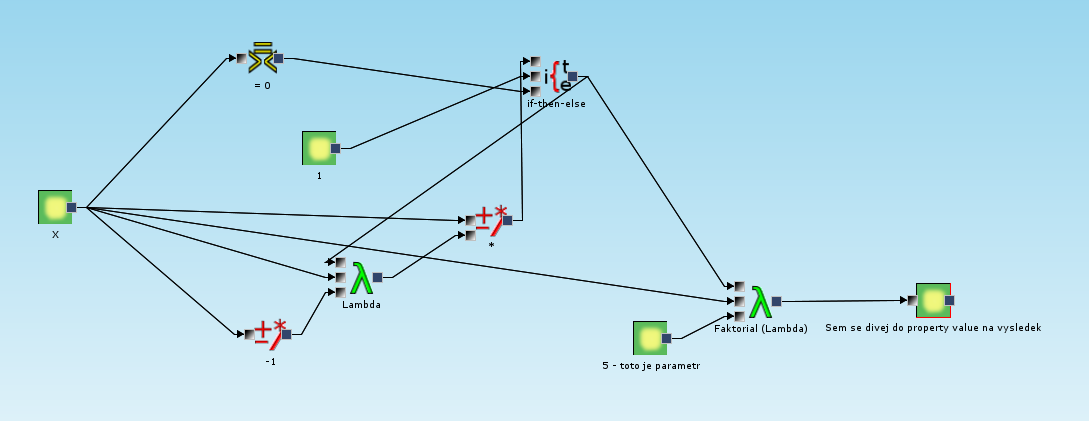
\includegraphics[width=1\textwidth]{faktorial}
	\caption{Factorial}
	\label{fig:factorial}
\end{figure}

When you are working with the lambda box in a recursion be aware of interminable function. For example if a user clicked on a plus box in the center of figure~\ref{fig:factorial}, the program would count infinitely, because the plus box has read-only property value and it should be set to $factorial(-1)$. The easy fix for this problem is to replace the condition $x=0$ with a condition $x<=0$. Because it is easy to create a interminable function and execute it, we prefer to save a project file very often.

\subsection{Sequences and sets}
\label{sec:sequences}
It is possible to represent a sequence of numbers by numbers only using basic primary recursive functions. But if there is a need of easy counting sequences of function it is better to add a support for that to the language.

The Ferda includes a box called Group. This box is the only box which is not the real back end module. It is implemented in the modules manager. It has one socked. It represents all boxes which are connected to this socket. If second group box is connected to this, the first box represents all boxes which are connected to the first box without the second group box but with all boxes which are represented by the second group box. If the box is connected to a socket to which it is possible to connect more boxes, it means all boxes which are represented by the box will be connected. The group box is very useful for organization of boxes on the desktop and reuse of a set of boxes.

We want to have a possibility to create a box which represents a sequence of boxes like the group box, but the box should be standard backend module. The box should return as a value a sequence of functions classes instead of one functions class. So we need second-order functions. It is easy thing in Ferda -- define a functions interface for sequence which has a methods which returns members of the sequence -- functions interfaces. Then a sequence boxes can be created. There are more ways how to define a sequence. For example one way is to have a box with property called ``count of items'' and when it is set to some number that number of socket will appear. These sockets represent items of a sequence. Another boxes can be ``head tail'' box (lisp and prolog use such ``functions''), ``clear sequence'',  ``add an item to the end'',\dots.

If a socket has an ability to connect more boxes, we can want a way how to connect all functions in some sequence to that socket. The implementation of connecting a box to a socked could be changed for that. A new implementation could first try if the functions is a sequence functions. If it was true, it would connect the functions interfaces inside the sequence, otherwise the functions interface itself.

The main implementation of a box module has a method which is used for getting of functions connected to some socket. It has this signature:
\begin{verbatim}
public ObjectPrx[] GetFunctions(string socketName)
\end{verbatim}

If the implementation can be changed so that if it is possible to connect more boxes to the socket ``socketName'', first try if the functions connected to that socket is a sequence. If it is true, do not return the sequence interface, but all functions which are in the sequence. In other scenarios the implementation should return the same result as it does.

Such change give us ability to use sequence boxes as a group box.

\subsubsection{ForEach box}
It can be very useful to have a box which gives a ability to create from one sequence other sequence the way that for each item in a sequence would be used the same function. We are going to call that new box ``ForEach''. It would have three sockets ``What'', ``Do'' and ``Variable''. Incoming sequence should be connected to the ``What'' socket. Function which changes the items should be connected to the ``Do'' socket. The function should use a variable which should be connected to the ``Variable'' socket. The variable will be replaced by items in the incoming sequence. Result is a sequence of cloned function where the variable was replaced by items in the incoming sequence. 

\subsection{Other new boxes}
\subsubsection{Get parameter}
!-- POPSAT --!
\begin{figure}
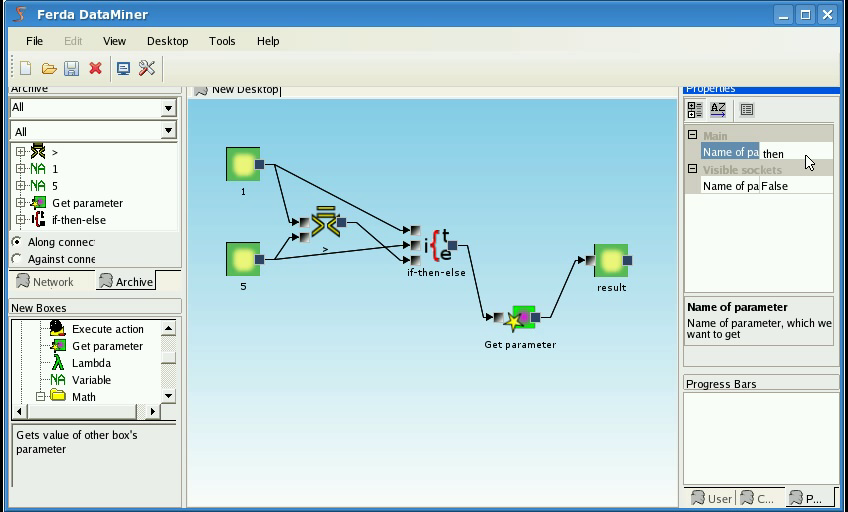
\includegraphics[width=1\textwidth]{getParameter2.png}
	\caption{Get parameter}
\end{figure}

\subsubsection{Execute action}
!-- POPSAT --!
\begin{figure}
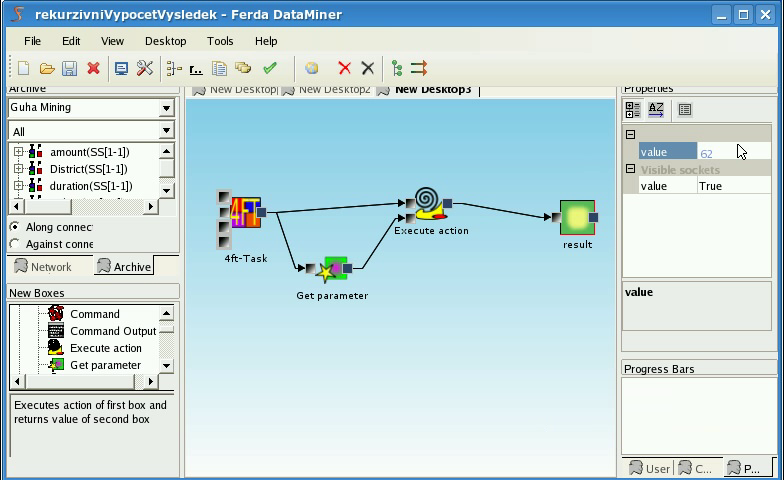
\includegraphics[width=1\textwidth]{executeAction2.png}
	\caption{Execute action}
\end{figure}

\subsubsection{Command and command output}
!-- POPSAT --!
\begin{figure}
	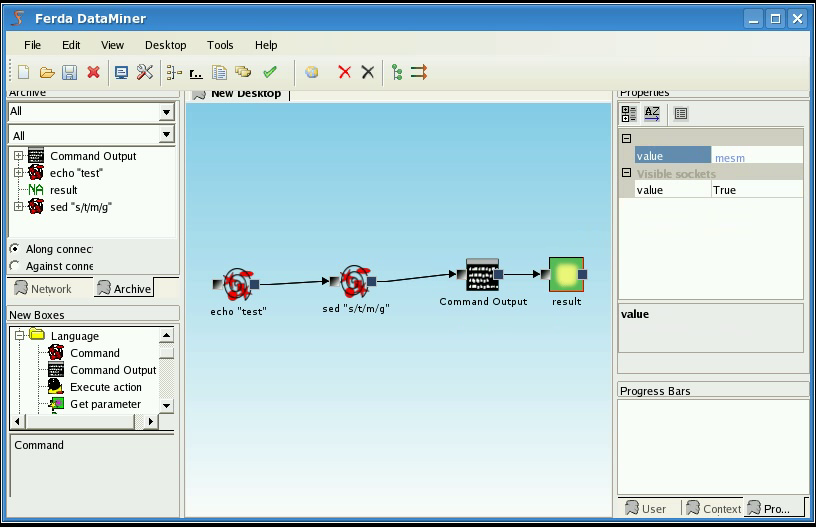
\includegraphics[width=1\textwidth]{command2.png}
	\caption{Command and command output}
\end{figure}

The same in console
\begin{figure}
	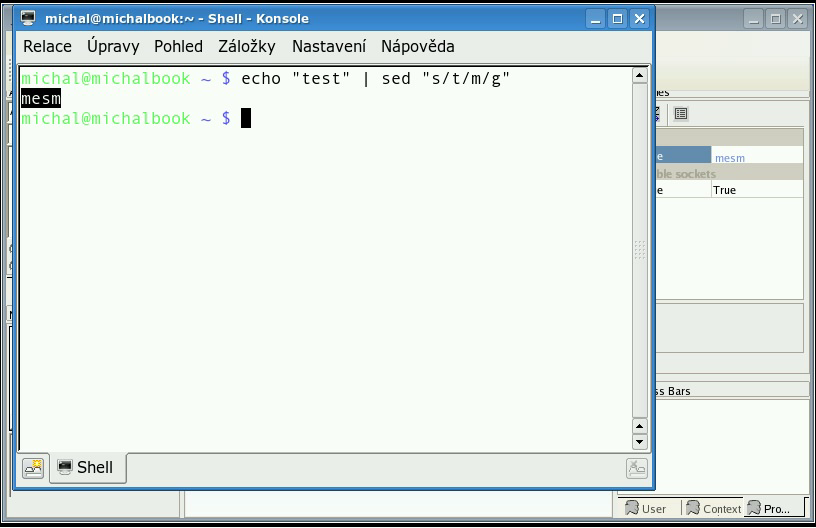
\includegraphics[width=1\textwidth]{command3.png}
	\caption{Konsole version previous example}
\end{figure}

\subsubsection{User-programmable box}
%TODO uzivatelsky programovatelna krabicka
!-- TODO uzivatelsky programovatelna krabicka -- programovani napriklad v pythonu krabicky za behu -- da se o tom napsat dost, trochu vetsi vykon nez programovani ve Ferdovi, ale zase nutna vetsi znalost, neni uplne trivialni implementovat \dots  --!


\section{Advanced tools and topics}
!-- TODO popsat o cem tato sekce je --!

\subsection{Unit tests}
It would be nice to have a box called unit test, which should have a name and one socket for connecting assert boxes. Assert box should be a box which validates some condition and when the condition is not satisfied it should return some message describing the problem. Then there should be small application which takes a project as parameter and calls all unit tests in the project. Unit tests should call all asserts which are connected to the test. When any of them fail the application should return the message with name of unit test and the error message from the failed assert. Even though one unit test failed it should call other tests.

Similar is the NUnit tool for .NET Framework. For reusing tools which executes NUnit tests it would be nice to create generator of NUnit tests from the Ferda project unit tests. Such generator should create one assembly for one project, but also so many test methods so many unit test boxes are in the project. There should be one startup method for initializing the Ferda Project Manager and for loading the project. 

\subsection{Exceptions}
!-- vyjimky a Ferda - uzivatel muze chytat a vysilat vyjimky --! U funkcialniho jazyka spise neco jako nedefinovana hodnota -- potreba porovnaatelnost s nedefinovatelnou hodnotou atd. Pokud nezbyde cas, sekci vynecham

\subsection{Dependency injection}
Dependency injection is modern pattern in object oriented programming. You create a services and specify which services depends on which interfaces and later you set if needed which instances should be used. It is very useful for unit testing. In Ferda we can see a box with all it's sub-boxes as a service. Not set sockets are interfaces on which it depends (because of lambda box it is not needed to define it on sub-boxes).

!-- dopsat --!

\subsection{Aspect oriented programming}

!-- možná zmínka, možná úplně odstraním --!

\subsection{Distributed computation}
!-- TODO vyber na kterem pocitaci ktera krabicka bezi pomoci propety gridu -- zmeni to Ferdu ve lepe distribuovany system, zajimave a ne moc tezke rozsireni --!

\chapter{KDD problems and theirs solutions}
\label{chap:KDDExamples}
This chapter shows data-mining examples and shows how it can be solved in the Ferda system by functionalities introduced in the first two chapters. It also proposes new functionalities specific for knowledge discovery.

\section{Four fold task in a recursion}
\subsection{Motivation}
Changes to a setting of a data-mining task is often needed after having a knowledge of results of the task. Subsequent run of that task can result in next changes of that settings. This step is repeated until the analytic is satisfied with the results or he gave up that setting at all.

!-- rozepsat nasledujici body ve vety --!

\begin{itemize}
			\item User tries some setting of quantifiers
			\item If he fails, he tries again with other settings?
			\item It's manual and confusing
\end{itemize}
		user wants
		\begin{itemize}
			\item find the best settings for task
			\item suggest way how to find best settings
			\item have for different tasks different methods
		\end{itemize}

It is possible that there can be known algorithm for a analytic how to change a setting after run of a task. Such information should be writable in the Ferda language.

Programming finding best settings by user -- biggest variability

Let us get a four fold task setting with founded implication quantifier. Generally, if the threshold of a founded implication is to hight, no results are returned by a task. If the threshold of a founded implication is to low many meaningless results are returned.

We will present small program in the new language which finds threshold for founded implication so that count of results of a task which use that quantifier is between specified numbers.

\subsection{Implementation}
The solution is based on the linear interpolation. The function of a count of results on a threshold is non-increasing. If we know two thresholds (the $x_{min}$ and the $x_{max}$) with their count of results (the $y_{min}$ and the $y_{max}$) which one count is shorter than what we wants and the second is greater than what we wants, than we can interpolate this way: 

\begin{math}
x = x_{max} - (y_{max} - y)\frac{x_{max} - x_{min}}{y_{max} - y_{min}}
\end{math}

$y$ is wanted count of results. Please see figure~\ref{fig:linearInterpolationPlot}. Such new $x$ is than lesser or equal to $x_{max}$ and greater or equal to $x_{min}$. Such computation would be repeated.

\begin{figure}
	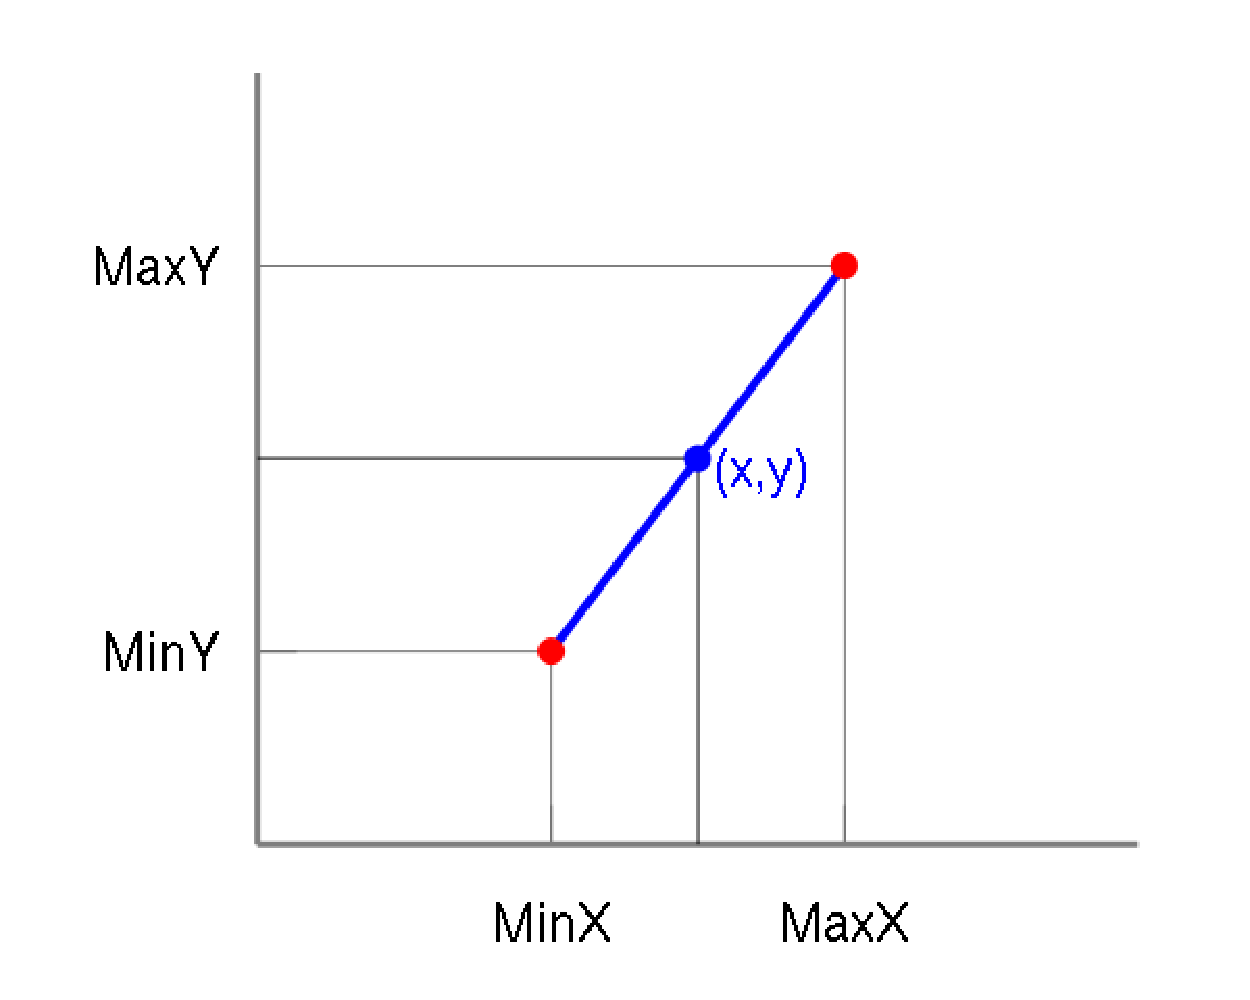
\includegraphics[width=1\textwidth]{linearInterpolationPlot}
	\caption{linear interpolation plot}
	\label{fig:linearInterpolationPlot}
\end{figure}

Because the function of a count of results on a threshold is not continuous we can not be sure that such interpolation founds wanted count of results. To overcame that the program will be satisfied with short interval instead of one number. In the actual example we are showing you, $y$ (wanted number of results) is set to five, but it will be satisfied if count of results will be between two and ten. It is still not enough, but it is simple and it helps. We can count in the program how deep it is in recursion and stop it after several steps if it will not find a sufficient result. But we will not do that for leaving the program simple as it can be. It's not hard to do that with the new language, you can try it as an exercise. 

The interpolation can be done in Ferda with the new box binary operation. Please see figure~\ref{fig:linearInterpolationBoxes}. Compare it with the equation above.

\begin{figure}
	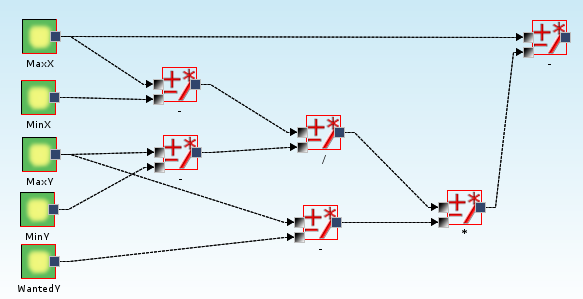
\includegraphics[width=1\textwidth]{linearInterpolation}
	\caption{interpolation as a connection of boxes}
	\label{fig:linearInterpolationBoxes}
\end{figure}

So the program will repetitively counts new threshold until it is satisfied. But which numbers should be on the beginning in the $x_{min}$, $x_{max}$, $y_{min}$ and $y_{max}$? Let us make decision that if a threshold is one, there are no results. It is true in standard situations. So, we can in the $x_{max}$ put one and in the $y_{max}$ put zero. Let us make second decision that if a threshold is zero, the number of results equals to ``max number of hypotheses'' parameter of the four fold task. So, we can put to the $x_{min}$ zero and to the $y_{min}$ put the same number as is in the ``max number of hypotheses'' parameter. Such thing can be best done by specifying that count only once in a integer box and connecting them to both ``max number of hypotheses'' socket and the socket of the ``MinY'' box.

At the beginning a threshold will be set to $0.5$. The program will first try to count number of hypotheses for that threshold. If the count is between two and ten the program returns that threshold.   

\begin{figure}
	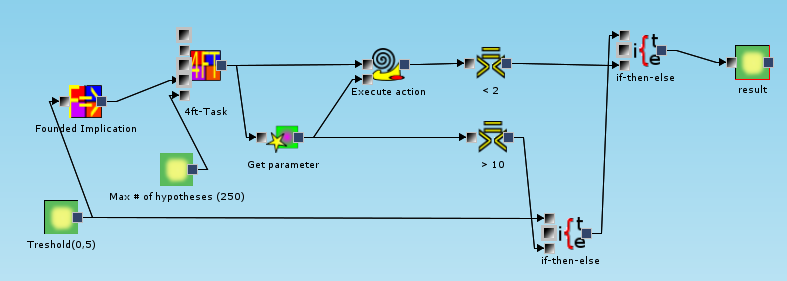
\includegraphics[width=1\textwidth]{exampleMainMiningPart}
	\caption{Basic of the recursive four fold example}
	\label{fig:basicRecursiveExample}
\end{figure}

Please see figure~\ref{fig:basicRecursiveExample}. The four boxes most on the left specify setting of the four fold task. The ``Get parameter'' box has set property ``ParameterName'' set to ``NumberOfHypotheses''. The ``Execute action'' box has set property ``ActionName'' set to ``Run''. It means that both these boxes returns number of hypotheses of the setting (they from point of value, because ``Get parameter'' box is connected to the ``Function'' socket of the box ``Execute action''). The ``Execute action'' also executes a searching for hypotheses in the setting. Without executing the action count of hypotheses can be invalid. So the action must be at least once executed. Two ``IfThenElse'' boxes with two ``Comparasion'' boxes in the figure returns the actual threshold if the number of hypotheses is between two and ten.

\begin{figure}
	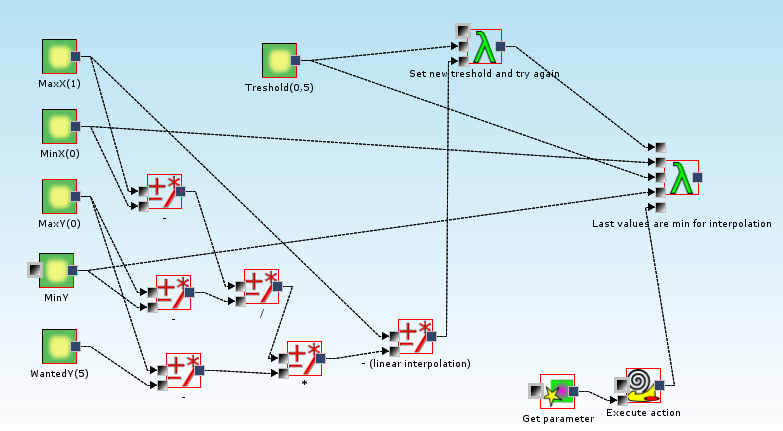
\includegraphics[width=1\textwidth]{exampleMainRecursionPart}
	\caption{Result should be between}
	\label{fig:resultBetween}
\end{figure}

It the number of hypotheses is lesser than two or greater than ten the program will count by interpolation a new threshold and executes this again. Please see figure~\ref{fig:resultBetween}. This is port of program variant where the count of hypotheses is greater than ten. In the interpolation $x_{min}$ will be set to the last threshold, $y_{min}$ will be set to last count of hypotheses. Than a new threshold will be counted by the interpolation and the result is again connected to the ``IfThenElse'' box from previous figure. You can see both two sub-connections together in figure~\ref{fig:exampleWithoutInterpolationOnMax}.

\begin{figure}
	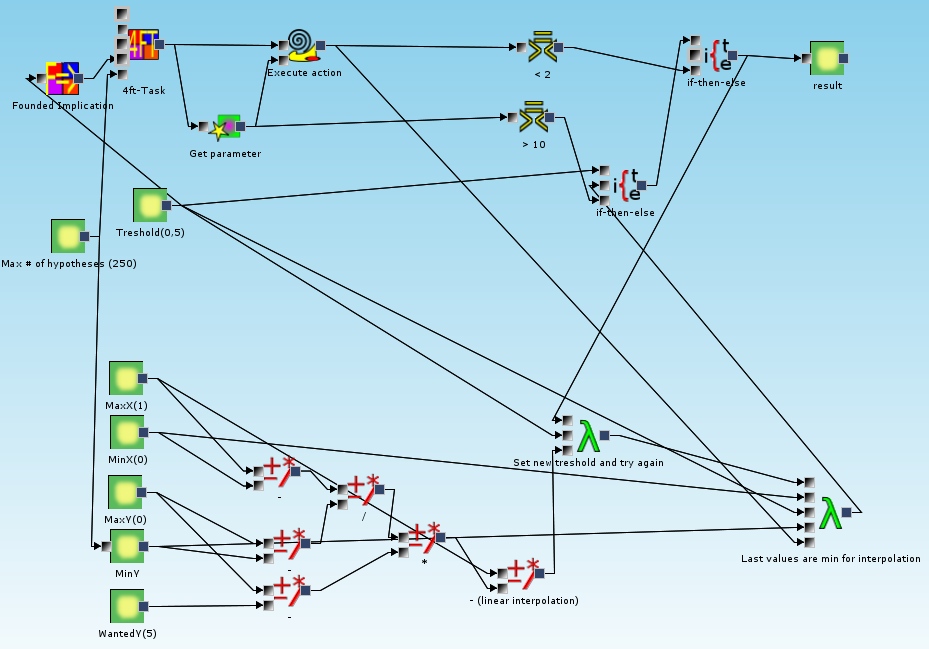
\includegraphics[width=1\textwidth]{exampleWithoutInterpolationOnMax}
	\caption{Example without $NumberOfHypotheses < 2$ part}
	\label{fig:exampleWithoutInterpolationOnMax}
\end{figure}

Whole program without details of four fold settings can be seen in figure~\ref{fig:exampleResult}. There is also part of program for variant where count of hypotheses is lesser than two. You can see that the connection do not look nice. It is because of many lines. Users can collapse boxes by packing feature of the FrontEnd. They can also use more desktops for organizing a program. A similar program in standard structural languages will not be easier.

\begin{figure}
	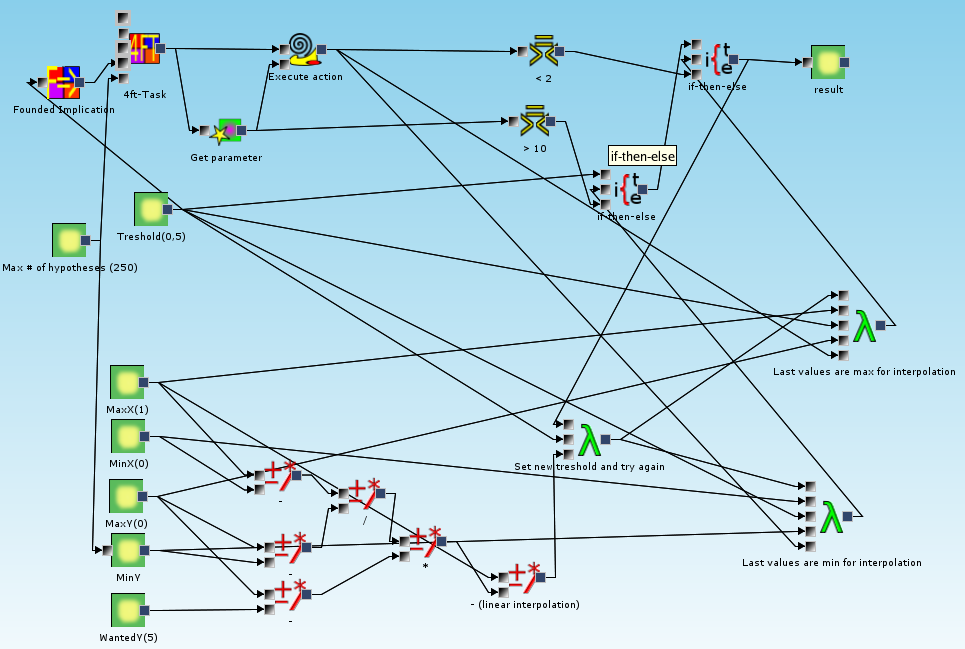
\includegraphics[width=1\textwidth]{exampleResult}
	\caption{Whole example}
	\label{fig:exampleResult}
\end{figure}

!-- TODO predelat obrazky ``Treshold'' na ``Threshold'', a misto ``Execute action'' snad muze byt zapojena do lambd krabicka ``Get parameter'' - tedy dost to zrychli pocitani (mozna je potreba jeste pres double box a je mi divne, ze bych to nezkousel -- mozna v tom je nejaky figl, zkusim) --!

\subsection{How to do it better}
The recursive computation is not needed for this particular task. The BestN algorithm for tasks, which is outlined in \cite{thesisKuchar}, can solve this particular task more effectively. But a user has to have a rich way how to specify best results. A functional language is a strong tool for such thing. We can see a functional language as a superset of observational calculus, which is described in~\cite{GUHAbook}. If we have only one quantifier, which is fuzzy, it is easy to sort results according goodness. For example, if we have only founded implication, a formula with higher threshold is the better. Founded implication is not today fuzzy, but we can easily convert it to that.

Two or more quantifiers as a setting for a task are more complicated. The today tasks accept a formula if all its quantifiers are satisfied. So the formula can be seen as a conjunction of the same subformulas only with a different quantifier. That conjunction is the real quantifier which is used in the GUHA mining. That conjunction should be used as a sorting filter for BestN. Today we have problem that the conjunction used is not a fuzzy conjunction. There is only one or zero. But there are many different fuzzy conjunctions and a user should have a ability to chose the right conjunction. He should be able to write his own conjuncti by the programming language.

There can be still more complicated tasks where the recursive solution described here can be useful.

\section{Getting basic information from a table}
Sometimes you get a data and do not know nearly anything about them. In such situations it would be convenient to have a method how to get quickly basic information about it.

A program which creates a basic generic settings from a table without any knowledge about it will be presented in this section. We will concentrate rather on a way how a user can create such program then on particular quantifiers, tasks and other properties of a setting which it should use.

Let us create a four fold task setting which in antecedent setting an atom setting created from any column of a table. So, the program should create an attribute for all columns in a table. It should decide a type of the attribute depending on a data in a column. Similarly, it should create an atom setting from the attribute. All these atom settings should be included in a cedent setting for the four fold task.

The program would create a sequence of atom settings for all columns. But first let us describe how would we write in Ferda a function which returns a sequence of all columns in a table. The table box type should have a new read-only property with names of columns. Today such information is returned by a method of a functions interface of the table box. The only way how to get such information from functions is by a custom box. If we had the new property with columns names, let us call it ``columns'', the GetParameter box could be used for getting such information as a parameter to next box. Such box we would use is the ForEach box.

\begin{eqnarray*}
ForEach(&&What=GetParameter(name="columns", box=Table(\dots)), \\&& Do=Column(name=X, table=Table(\dots)), \\&& Variable=X)
\end{eqnarray*}

This connection returns a sequence of columns. The $X$ can represent for example $String()$ or $Variable()$.

The second task is to create attribute in dependency on a column. If a column had more then 20 distinct values the equifrequency attribute would be used otherwise the each value one category attribute would be used. Let us call a column in previus connection $C$

\begin{eqnarray*}
C=Column(name=X, table=Table(\dots))
\end{eqnarray*}

Than if we changed in the last connection in the ForEach box the connection to the ``Do'' socket this way

\begin{eqnarray*}
Do=IfThenElse(&&Comparasion(type="<=", \\&&\qquad value1=GetParameter(name="distinctValues", \\&&\qquad\qquad box=C), \\&&\qquad value2=20),\\&&Atom(EachValueOneAttribute(column=C,\dots)),\\&&Atom(EquifrequencyAttribute(column=C,\dots)))
\end{eqnarray*}

result of such connection would be the wanted sequence of atom settings. Such sequence could be connected to a cedent box, that box could be than connected as both an antecedent and a succedent of a four fold task.

\section{GUHA in Ferda by ``small'' boxes}
%Implementation of GUHA in Ferda by 'small' boxes.
!-- jak delat programove sekvence hopotez a resit je pomoci specifickeho GUHA solveru -- vetsi sire nez soucasna implementace (lze hledat nejen formule specifickeho tvaru ale obecne jakekoliv formule), ale samozrejme daleko pomalejsi --!

!-- souvisi result browser - aby umel heterogenni vysledky - vystup z 4FT + vystup z CF --!

\section{\dots}
\chapter{Summary}
The thesis has described a new language for a data mining. It is a visual functional language. Functions are there called boxes. Basic formalisation of the language has been shown in the section~\ref{sec:formalisation}. A source code is written as a connection of boxes, source files are project files of the Ferda system. Possible extensions to source files has been described in the section~\ref{sec:reusability}. These extensions adds better reusability of a code. One such extension, which is called ``network archive'' has been implemented as part of this thesis. Future possible enhancement to the network archive has been also proposed.

A basic set of boxes has been created as part of the thesis and other boxes has been proposed. The boxes which has been created includes the constant boxes, the BinaryOperation box, the Comparison box, the IfThenElse box, the Lambda box, the GetParameter box, the ExecuteAction box, the Command box and the CommandOutput box. The most complicated box from these is the Lambda box. There has been discussed several problems of the box and their possible solutions. The boxes which has been only proposed includes different sequence boxes, the ForEach box and the user-programmable box.

The three examples of the usage of the new language for data-mining has been shown. The first example introduces a recursive computation of data mining tasks. An implementation of that example is part of this thesis. The second example shows how can be created with the proposed language a generic setting which gets basic information about data in any table. The third example presents a more generic implementation of GUHA based on simple boxes.

%\section{Future tasks to do in Ferda}
%popis jednotlivych tasku s narocnosti, uzitkem - bodove ohodnotit

% modules for interacion je treba vylepsit

%\bibliographystyle{abbrv}
%\bibliographystyle{czechiso}
%\bibliographystyle{plain}

\bibliographystyle{cj}
\bibliography{thesis}

%\begin{thebibliography}{thesisKuchar}
%\bibitem{GMGC} Rauch J., Šimůnek M.: GUHA Method and Granular Computing. In: Hu X., Liu Q., Skowron A., Lin T. Y., Yager R., Zang B. (ed.). Proceedings of IEEE konference Granular Computing 2005. Piscataway: IEEE, 2005, s. 630–635. ISBN 0-7803-9017-2.
%\bibitem{thesisKuchar} Tomáš Kuchař -- jeho diplomová práce
%\bibitem{GUHAbook} GUHA book
%\bibitem{znalosti2006} Kováč M., Kuchař T., Kuzmin A., Ralbovský M.: Ferda, nové vizuální prostředí pro dobývání znalostí. Přijato k prezentaci na konferenci ZNALOSTI 2006, viz http://fim.uhk.cz/znalosti/index.php?p=prispevky
%\bibitem{Ice} Internet Communications Engine documentation
%\bibitem{Wiki} linearni interpolace 
%\bibitem{dalsi} \dots
%\end{thebibliography}
\end{document}
